\chapter{Theory of the Plasma Sheath}
\label{ch:sheath}

Every laboratory or technological plasma is bounded by a material surface, and it is at that boundary that the plasma communicates its energy, particle, and momentum content to the outside world. The layer that mediates this communication is the \emph{sheath}: a thin, non-neutral region, typically a few to a few tens of Debye lengths thick, in which the plasma potential collapses from its quasineutral bulk value to the (generally more negative) value imposed by the wall. Because essentially all of the potential drop between the plasma interior and a solid boundary occurs across this narrow layer, the sheath determines the energy with which ions strike a surface -- the ion energy flux $\Gamma_{E}$ this monograph quantifies. This chapter develops sheath theory from first principles: why a sheath must exist, the Bohm criterion and presheath that enforce it, the space-charge-limited sheath structure (matrix and Child--Langmuir limits), its generalization to collisional and magnetized plasmas (the Bohm--Chodura criterion), its time-dependent behaviour under RF excitation, and the kinetic and finite-Debye-length corrections that refine the fluid picture. The notation $T_{\mathrm{e}}$, $T_{\mathrm{i}}$, $n_{\mathrm{e}}$, $n_{\mathrm{i}}$, $\lambda_{\mathrm{D}}$, $u_{\mathrm{B}}$, $\Gamma_{E}$, $f_{\mathrm{i}}(v)$ is used consistently throughout.

\section{Why a Sheath Forms: Differential Mobility and Flux Balance}

\subsection{The disparity in thermal velocities}

The physical origin of the sheath lies in the disparity between electron and ion thermal velocities in a weakly ionized, low-temperature plasma. For a Maxwellian species of mass $m$ and temperature $T$, the mean thermal speed is
\begin{equation}
\bar{v} = \sqrt{\frac{8 k_{\mathrm{B}} T}{\pi m}},
\end{equation}
and the random one-sided flux incident on a plane surface from an isotropic Maxwellian distribution is $\Gamma = \tfrac{1}{4} n \bar{v}$. Because $m_{\mathrm{i}} \gg m_{\mathrm{e}}$ (a factor of $\num{1836}$ for hydrogen, up to $\sim \num{2.4e5}$ for xenon) and $T_{\mathrm{e}} \gtrsim T_{\mathrm{i}}$ in most laboratory discharges, electrons are vastly more mobile than ions. If a plasma with $n_{\mathrm{e}} = n_{\mathrm{i}}$ were suddenly placed in contact with a floating or grounded wall, the initial electron flux would exceed the ion flux by a factor of order $\sqrt{m_{\mathrm{i}}/m_{\mathrm{e}}}$, two to three orders of magnitude -- the starting point for essentially every treatment of the plasma-sheath transition \cite{ref0013,ref0015}.

\subsection{Charge accumulation and the self-consistent field}

Because electrons escape to the wall far faster than ions, the wall rapidly accumulates net negative charge, while the adjacent plasma is left correspondingly positive as it is depleted of electrons. The resulting field points from the quasineutral bulk toward the wall, decelerating fast electrons and accelerating slow ions, until a steady state is reached in which the depressed electron flux balances the enhanced ion flux. The layer that carries this field, and the compensating charge deficit required by Poisson's equation, is the sheath -- a direct consequence of flux balance under a large electron-to-ion mobility ratio.

\subsection{Quasineutrality breakdown and the natural length scale}

In the bulk plasma, quasineutrality ($n_{\mathrm{e}} \simeq n_{\mathrm{i}}$) is maintained to high precision: any local charge imbalance $\delta n = n_{\mathrm{i}} - n_{\mathrm{e}}$ produces, through Poisson's equation,
\begin{equation}
\nabla^{2} \phi = -\frac{e\,\delta n}{\varepsilon_{0}},
\end{equation}
a restoring field acting on a length scale set by the electron Debye length,
\begin{equation}
\lambda_{\mathrm{D}} = \left( \frac{\varepsilon_{0} k_{\mathrm{B}} T_{\mathrm{e}}}{n_{\mathrm{e}} e^{2}} \right)^{1/2}.
\label{ch03-eq:debye-length}
\end{equation}
Over distances much larger than $\lambda_{\mathrm{D}}$ the plasma shields out imposed potential perturbations and remains quasineutral; on distances comparable to or smaller than $\lambda_{\mathrm{D}}$, quasineutrality can fail, since the electrostatic energy of charge separation becomes comparable to the particle thermal energy. The sheath is where this failure is enforced by the boundary condition itself: the wall must absorb net negative charge to establish the retarding potential that balances the fluxes, so Poisson's equation requires $n_{\mathrm{i}} > n_{\mathrm{e}}$ throughout. The natural thickness of this layer is of order a few $\lambda_{\mathrm{D}}$ in the simplest (``matrix'') approximation, growing super-linearly with voltage once ion space charge is treated self-consistently (the Child--Langmuir regime) \cite{ref0012,ref0024}.

\section{Plasma, Wall, and Floating Potentials}

\subsection{Definitions and the current-balance framework}

Three potentials organize the discussion of any bounded plasma. The \emph{plasma potential} $V_{\mathrm{p}}$ is the potential of the quasineutral bulk, the reference for all sheath potential drops. The \emph{wall potential} $V_{\mathrm{w}}$ is the potential actually acquired by the bounding surface, depending on whether it is floating, grounded, or externally biased. The \emph{floating potential} $V_{\mathrm{f}}$ is the special case realized when the surface draws no net current -- the condition defining a probe or any unbiased dielectric wall. In all cases the physics is governed by the total current density delivered to the surface,
\begin{equation}
J(V_{\mathrm{w}}) = J_{\mathrm{i}}(V_{\mathrm{w}}) - J_{\mathrm{e}}(V_{\mathrm{w}}),
\end{equation}
with $J_{\mathrm{i}}$ and $J_{\mathrm{e}}$ both defined positive when directed toward the wall.

\subsection{Ion and electron current density at the surface}

The ion current density delivered to the wall is fixed by the flux of ions crossing the sheath edge -- set by the Bohm criterion of Section~\ref{ch03-sec:bohm}, essentially independent of $V_{\mathrm{w}}$ provided $V_{\mathrm{w}} < V_{\mathrm{p}}$:
\begin{equation}
J_{\mathrm{i}} = e\, n_{\mathrm{s}}\, u_{\mathrm{B}}, \qquad u_{\mathrm{B}} = \sqrt{\frac{k_{\mathrm{B}} T_{\mathrm{e}}}{m_{\mathrm{i}}}},
\label{eq:bohm-flux}
\end{equation}
where $n_{\mathrm{s}}$ is the sheath-edge density and $u_{\mathrm{B}}$ the Bohm speed. The electron current, by contrast, is exponentially sensitive to the retarding potential, since only the high-energy tail with $\tfrac12 m_{\mathrm{e}} v^{2} \geq e|V_{\mathrm{p}} - V_{\mathrm{w}}|$ surmounts the barrier:
\begin{equation}
J_{\mathrm{e}}(V_{\mathrm{w}}) = \frac{1}{4} e\, n_{\mathrm{s}} \bar{v}_{\mathrm{e}} \exp\!\left[ \frac{e (V_{\mathrm{w}} - V_{\mathrm{p}})}{k_{\mathrm{B}} T_{\mathrm{e}}} \right], \qquad \bar{v}_{\mathrm{e}} = \sqrt{\frac{8 k_{\mathrm{B}} T_{\mathrm{e}}}{\pi m_{\mathrm{e}}}}.
\label{eq:electron-retarded-flux}
\end{equation}
This exponential form recurs in the presheath and is central to virtually every fluid derivation of the Bohm criterion \cite{ref0013}.

\subsection{The floating condition}

The floating potential is obtained by setting $J = 0$, i.e.\ equating the retarded electron flux of Eq.~\eqref{eq:electron-retarded-flux} to the Bohm ion flux of Eq.~\eqref{eq:bohm-flux}:
\begin{equation}
\frac{1}{4} \bar{v}_{\mathrm{e}} \exp\!\left[ \frac{e (V_{\mathrm{f}} - V_{\mathrm{p}})}{k_{\mathrm{B}} T_{\mathrm{e}}} \right] = u_{\mathrm{B}}.
\end{equation}
Solving for the sheath potential drop gives the classical floating-potential formula
\begin{equation}
V_{\mathrm{f}} - V_{\mathrm{p}} = -\frac{k_{\mathrm{B}} T_{\mathrm{e}}}{2e} \ln\!\left( \frac{m_{\mathrm{i}}}{2\pi m_{\mathrm{e}}} \right).
\label{eq:floating-potential}
\end{equation}
Because $m_{\mathrm{i}}/m_{\mathrm{e}} \gg 1$ for any real ion, the logarithm is positive and of order $5$--$10$, so the floating surface always sits several electron temperatures below the plasma potential. Table~\ref{tab:floating-potentials} lists the normalized offset for several ion species; it grows slowly (logarithmically) with ion mass.

\begin{table}[htbp]
\centering
\caption{Normalized floating-potential offset $-(V_{\mathrm{f}} - V_{\mathrm{p}})/T_{\mathrm{e}}$ from Eq.~\eqref{eq:floating-potential} for representative singly ionized species (cold-ion limit, $T_{\mathrm{i}} \to 0$); values are illustrative, computed from the analytic formula, not measurements.}
\label{tab:floating-potentials}
\begin{tabular}{lcc}
\toprule
Ion species & $m_{\mathrm{i}}/m_{\mathrm{e}}$ & $-(V_{\mathrm{f}}-V_{\mathrm{p}})/T_{\mathrm{e}}$ \\
\midrule
Hydrogen (H$^{+}$) & $1.84\times10^{3}$ & $2.84$ \\
Helium (He$^{+}$) & $7.34\times10^{3}$ & $3.53$ \\
Argon (Ar$^{+}$) & $7.34\times10^{4}$ & $4.68$ \\
Xenon (Xe$^{+}$) & $2.41\times10^{5}$ & $5.28$ \\
\bottomrule
\end{tabular}
\end{table}

For $V_{\mathrm{w}} < V_{\mathrm{f}}$, the ion current saturates at the Bohm value while the electron current falls exponentially -- the regime governing ion energy delivered to any negatively biased surface.

\subsection{Grounded and biased surfaces}

When $V_{\mathrm{w}}$ is fixed externally -- a grounded electrode, a DC- or RF-biased substrate -- the net current need not vanish, and $V_{\mathrm{p}} - V_{\mathrm{w}}$ becomes the controlling parameter for ion bombardment energy. Since this drop occurs almost entirely across the sheath (the presheath drop being only $T_{\mathrm{e}}/2e$), an ion entering at $u_{\mathrm{B}}$ and falling through the full sheath potential arrives with kinetic energy
\begin{equation}
E_{\mathrm{i}} \simeq \frac{1}{2} m_{\mathrm{i}} u_{\mathrm{B}}^{2} + e\left(V_{\mathrm{p}} - V_{\mathrm{w}}\right) = \frac{1}{2} k_{\mathrm{B}} T_{\mathrm{e}} + e\left(V_{\mathrm{p}} - V_{\mathrm{w}}\right),
\label{eq:ion-impact-energy}
\end{equation}
in the collisionless, unidirectional limit. Equation~\eqref{eq:ion-impact-energy} is the fundamental link between sheath theory and the ion energy flux $\Gamma_{E} = \Gamma_{\mathrm{i}} E_{\mathrm{i}}$ this monograph quantifies, and is refined below to account for collisions, magnetization, time dependence, and the finite spread of $f_{\mathrm{i}}(v)$.

\subsection{The ion energy flux as a moment of the sheath-edge distribution}

Given the ion velocity distribution $f_{\mathrm{i}}(v)$ at any plane of interest -- most usefully the wall -- the ion particle flux and ion energy flux are the zeroth and energy-weighted first moments of $f_{\mathrm{i}}(v)$:
\begin{equation}
\Gamma_{\mathrm{i}} = \int_{0}^{\infty} v\, f_{\mathrm{i}}(v)\, \mathrm{d}v, \qquad \Gamma_{E} = \int_{0}^{\infty} \left( \frac{1}{2} m_{\mathrm{i}} v^{2} \right) v\, f_{\mathrm{i}}(v)\, \mathrm{d}v.
\label{eq:energy-flux-moments}
\end{equation}
In the idealized cold-ion, collisionless, unmagnetized, DC limit, $f_{\mathrm{i}}(v)$ collapses to a delta function at the impact speed of Eq.~\eqref{eq:ion-impact-energy}, and Eq.~\eqref{eq:energy-flux-moments} reduces to $\Gamma_{E} = \Gamma_{\mathrm{i}} E_{\mathrm{i}}$. Every generalization treated below -- collisional broadening, the Bohm--Chodura conditions, the bimodal RF distribution, and the kinetic Bohm criterion of Eq.~\eqref{eq:kinetic-bohm} -- broadens, skews, or splits $f_{\mathrm{i}}(v)$ away from this delta function, decoupling $\Gamma_{E}$ from the simple product of mean flux and mean energy. Because $\Gamma_{E}$ weights by an extra factor of $v^{2}$, it is disproportionately sensitive to the high-energy tail of $f_{\mathrm{i}}(v)$, in contrast to the kinetic Bohm criterion (Section~\ref{ch03-sec:bohm}), whose $v^{-2}$ weighting makes it sensitive to the low-energy tail: a population can satisfy the marginal Bohm condition comfortably in bulk while its low-velocity tail threatens it, yet deliver an energy flux dominated by a high-velocity tail representing a small fraction of the total flux. Quantifying $\Gamma_{E}$ accurately therefore requires the full shape of $f_{\mathrm{i}}(v)$, not merely the mean sheath voltage and Bohm flux.

\section{The Bohm Criterion and the Presheath}
\label{ch03-sec:bohm}

\subsection{Statement and fluid model}

The Bohm criterion is the single most important quantitative result in sheath theory: ions cannot enter a sheath at rest, or even at an arbitrary subsonic drift, but must arrive at the sheath edge with directed velocity at least the ion acoustic (Bohm) speed $u_{\mathrm{B}} = \sqrt{k_{\mathrm{B}} T_{\mathrm{e}}/m_{\mathrm{i}}}$, first obtained by Bohm and later elaborated into kinetic, collisional, multi-species, and magnetized forms \cite{ref0001,ref0004}. It follows from requiring a monotonic, physically admissible space-charge solution of Poisson's equation between the quasineutral plasma and the strongly non-neutral sheath.

Consider a one-dimensional, steady-state, cold-ion fluid model: ions are created far from the wall and fall collisionlessly and unmagnetized through the presheath and sheath, while electrons, Maxwellian at $T_{\mathrm{e}}$, obey the Boltzmann relation at every point:
\begin{equation}
n_{\mathrm{e}}(\phi) = n_{0} \exp\!\left( \frac{e \phi}{k_{\mathrm{B}} T_{\mathrm{e}}} \right),
\label{ch03-eq:electron-boltzmann}
\end{equation}
where $\phi \le 0$ is the local potential relative to the field-free interior and $n_{0}$ the unperturbed bulk density. Ion continuity and cold-ion momentum conservation give
\begin{align}
n_{\mathrm{i}}(x)\, u_{\mathrm{i}}(x) &= \Gamma_{\mathrm{i}} = n_{0} u_{0}, \label{eq:ion-continuity}\\
\frac{1}{2} m_{\mathrm{i}} u_{\mathrm{i}}^{2}(x) &= \frac{1}{2} m_{\mathrm{i}} u_{0}^{2} - e \phi(x), \label{eq:ion-energy}
\end{align}
where $u_{0}$ is the ion drift speed at the presheath--sheath reference point $\phi=0$. Combining these yields the ion density profile
\begin{equation}
n_{\mathrm{i}}(\phi) = \frac{n_{0} u_{0}}{\sqrt{u_{0}^{2} - 2 e \phi/m_{\mathrm{i}}}}.
\label{eq:ion-density-profile}
\end{equation}

\subsection{Poisson's equation and the marginal stability argument}

The self-consistent potential must satisfy Poisson's equation with the two charge densities of Eqs.~\eqref{ch03-eq:electron-boltzmann} and~\eqref{eq:ion-density-profile}:
\begin{equation}
\varepsilon_{0} \frac{\mathrm{d}^{2} \phi}{\mathrm{d} x^{2}} = e \left[ n_{\mathrm{e}}(\phi) - n_{\mathrm{i}}(\phi) \right] = e n_{0} \left[ \exp\!\left(\frac{e\phi}{k_{\mathrm{B}} T_{\mathrm{e}}}\right) - \frac{u_{0}}{\sqrt{u_{0}^{2} - 2e\phi/m_{\mathrm{i}}}} \right].
\label{ch03-eq:poisson-full}
\end{equation}
For a physically sensible solution, in which $\phi$ decreases monotonically from $0$ to a negative wall value, the right-hand side must be non-negative for all $\phi\le0$ near $\phi=0$. Expanding both terms to first order in $\phi$,
\begin{align}
n_{\mathrm{e}}(\phi) &\approx n_{0}\left(1 + \frac{e\phi}{k_{\mathrm{B}} T_{\mathrm{e}}}\right), &
n_{\mathrm{i}}(\phi) &\approx n_{0}\left(1 + \frac{e\phi}{m_{\mathrm{i}} u_{0}^{2}}\right),
\end{align}
and substituting into Eq.~\eqref{ch03-eq:poisson-full}, the linear term gives
\begin{equation}
\varepsilon_{0} \frac{\mathrm{d}^{2}\phi}{\mathrm{d} x^{2}} \approx e n_{0}\, \phi\left( \frac{1}{k_{\mathrm{B}} T_{\mathrm{e}}} - \frac{1}{m_{\mathrm{i}} u_{0}^{2}} \right).
\label{eq:linearized-poisson}
\end{equation}
Since $\phi\le0$, the bracketed term must be non-negative for net positive space charge:
\begin{equation}
\frac{1}{k_{\mathrm{B}} T_{\mathrm{e}}} \ge \frac{1}{m_{\mathrm{i}} u_{0}^{2}} \qquad \Longleftrightarrow \qquad u_{0}^{2} \ge \frac{k_{\mathrm{B}} T_{\mathrm{e}}}{m_{\mathrm{i}}},
\end{equation}
which on taking the square root gives the Bohm criterion,
\begin{equation}
\boxed{\, u_{0} \ge u_{\mathrm{B}} \equiv \sqrt{\frac{k_{\mathrm{B}} T_{\mathrm{e}}}{m_{\mathrm{i}}}} \,}.
\label{ch03-eq:bohm-criterion}
\end{equation}
Eq.~\eqref{ch03-eq:bohm-criterion} is a marginal (inequality) condition rather than an exact equality: if $u_0 < u_{\mathrm B}$, no monotonic space-charge solution exists; if $u_0 = u_{\mathrm B}$ exactly, the linear term vanishes and higher-order terms must sustain the field, producing a formally singular ion density gradient at the sheath edge.

\subsection{Physical interpretation}

The Bohm criterion can be read as a statement about the relative stiffness of ion and electron responses to a potential perturbation. From Eq.~\eqref{eq:linearized-poisson}, $1/(m_{\mathrm{i}} u_{0}^{2})$ is the ion compressibility response and $1/(k_{\mathrm{B}} T_{\mathrm{e}})$ the electron (Boltzmann) response to the same $\phi$. When ions are slow, a small negative $\phi$ compresses the ion fluid more strongly than it depletes the electrons, so $n_{\mathrm{i}} > n_{\mathrm{e}}$ is never achieved; once ions move fast enough, further deceleration produces only a small density increase, while the exponential electron response keeps depleting $n_{\mathrm{e}}$, letting the required space charge build. The Bohm speed is thus the threshold ion drift at which the ion fluid becomes ``stiff'' enough, relative to the electrons, to support a stable non-neutral transition.

\subsection{The presheath}

The Bohm criterion demands that ions arrive at the sheath edge already moving at $u_{\mathrm{B}}$, yet ions are typically born by ionization essentially at rest. The region that performs this acceleration is the \emph{presheath}: a quasineutral region, generally many Debye lengths in extent, supporting a weak field that accelerates ions from rest up to $u_{\mathrm{B}}$ while remaining quasineutral to good approximation \cite{ref0006,ref0013}. The total presheath potential drop follows from Eq.~\eqref{eq:ion-energy} between the field-free source ($u\approx0$) and the sheath edge ($u=u_{\mathrm{B}}$):
\begin{equation}
e \left| \Delta \phi_{\mathrm{presheath}} \right| = \frac{1}{2} m_{\mathrm{i}} u_{\mathrm{B}}^{2} = \frac{1}{2} k_{\mathrm{B}} T_{\mathrm{e}} \qquad \Longrightarrow \qquad \Delta\phi_{\mathrm{presheath}} = -\frac{k_{\mathrm{B}} T_{\mathrm{e}}}{2e}.
\label{eq:presheath-drop}
\end{equation}
This universal result -- a presheath drop of exactly $T_{\mathrm{e}}/2$ for cold, unmagnetized, collisionless ions born at rest -- is a direct corollary of the Bohm criterion \cite{ref0013,ref0023}. The associated sheath-edge density reduction follows from Eq.~\eqref{ch03-eq:electron-boltzmann}: $n_{\mathrm{s}} = n_{0} \exp(-1/2) \approx 0.61\, n_{0}$, a factor used throughout plasma diagnostics to relate a bulk density measurement to the flux delivered to a wall.

The presheath/sheath boundary is not a sharp physical division but a matter of scale separation -- the presheath varies on the ionization or collisional mean free path, the sheath on the Debye length -- formally distinct only as $\lambda_{\mathrm{D}} \to 0$; what condition to impose at the notional sheath edge remains debated.

\section{Sheath Structure and Thickness}

\subsection{Debye-length scaling of the collisionless sheath}

Once ions cross the sheath edge at $u_{\mathrm{B}}$, they enter a region where quasineutrality is abandoned and the full nonlinear Poisson equation, Eq.~\eqref{ch03-eq:poisson-full}, governs the potential profile. Two limiting, tractable descriptions are standard: the \emph{matrix sheath}, appropriate to an initial transient or order-of-magnitude estimate, and the \emph{Child--Langmuir sheath}, appropriate to a steady, voltage-driven sheath where ion density has fallen substantially by the wall. Both predict a thickness of order a few Debye lengths for $V_{0} \sim T_{\mathrm{e}}$, growing as a power of the voltage at larger bias \cite{ref0012,ref0024}.

\subsection{The matrix sheath}

The matrix-sheath approximation sets $n_{\mathrm{i}}(x) = n_{\mathrm{s}}$ uniformly and neglects the electron density ($n_{\mathrm{e}} \approx 0$, exponentially small once $|\phi| \gg T_{\mathrm{e}}/e$). Poisson's equation becomes linear in $x$:
\begin{equation}
\varepsilon_{0} \frac{\mathrm{d}^{2}\phi}{\mathrm{d}x^{2}} = -e\, n_{\mathrm{s}}.
\end{equation}
Taking the sheath edge at $x=0$ with $\phi(0)=0$ and $\mathrm{d}\phi/\mathrm{d}x|_{x=0}=0$, integration gives
\begin{equation}
\phi(x) = -\frac{e n_{\mathrm{s}}}{2\varepsilon_{0}} x^{2}.
\end{equation}
Setting $\phi(s) = -V_{0}$ at the wall ($V_{0} = V_{\mathrm{p}} - V_{\mathrm{w}} > 0$) and solving for $s$ gives the matrix-sheath thickness
\begin{equation}
s_{\mathrm{matrix}} = \left( \frac{2 \varepsilon_{0} V_{0}}{e n_{\mathrm{s}}} \right)^{1/2} = \lambda_{\mathrm{Ds}} \left( \frac{2 e V_{0}}{k_{\mathrm{B}} T_{\mathrm{e}}} \right)^{1/2},
\label{eq:matrix-sheath}
\end{equation}
where $\lambda_{\mathrm{Ds}} = (\varepsilon_{0} k_{\mathrm{B}} T_{\mathrm{e}} / n_{\mathrm{s}} e^{2})^{1/2}$ is the Debye length at the sheath-edge density: a few Debye lengths for $V_{0}$ of order a few $T_{\mathrm{e}}$, growing only as the square root of the applied voltage.

\subsection{The Child--Langmuir sheath}

The matrix approximation over-estimates ion density (and under-estimates thickness) at large voltage, since it ignores that ions accelerate substantially crossing the sheath, so $n_{\mathrm{i}}(x)$ must fall with distance to keep $\Gamma_{\mathrm{i}} = n_{\mathrm{i}} u_{\mathrm{i}}$ constant. Retaining this gives the space-charge-limited, or Child--Langmuir, sheath. With $x=0$, $\phi(0)=0$, and $u_{\mathrm{i}}(0)=u_{\mathrm{B}}$ (negligible for $V_0 \gg T_{\mathrm{e}}/e$, dropped below), current continuity and energy conservation give
\begin{equation}
J_{\mathrm{i}} = e\, n_{\mathrm{i}}(x)\, u_{\mathrm{i}}(x) = \text{const}, \qquad \frac{1}{2} m_{\mathrm{i}} u_{\mathrm{i}}^{2}(x) = -e\phi(x) \equiv e\,\psi(x),
\end{equation}
with $\psi \equiv -\phi \ge 0$ rising monotonically from $0$ at the sheath edge to $V_{0}$ at the wall. Eliminating $u_{\mathrm{i}}$ gives $n_{\mathrm{i}}(x) = J_{\mathrm{i}} / [e \sqrt{2e\psi/m_{\mathrm{i}}}\,]$, and neglecting the electron density in the sheath interior, Poisson's equation becomes
\begin{equation}
\varepsilon_{0} \frac{\mathrm{d}^{2}\psi}{\mathrm{d}x^{2}} = J_{\mathrm{i}} \sqrt{\frac{m_{\mathrm{i}}}{2 e \psi}}.
\label{eq:cl-ode}
\end{equation}
Integrating once (with $\mathrm{d}\psi/\mathrm{d}x=0$ at $x=0$) gives $\mathrm{d}\psi/\mathrm{d}x = \left[ (4 J_{\mathrm{i}}/\varepsilon_{0}) \sqrt{m_{\mathrm{i}}/2e} \right]^{1/2} \psi^{1/4}$; integrating again from $\psi=0$ at $x=0$ gives $\tfrac{4}{3}\psi^{3/4} = \left[ (4J_{\mathrm{i}}/\varepsilon_{0})\sqrt{m_{\mathrm{i}}/2e} \right]^{1/2} x$. Evaluating at the wall, $\psi(s)=V_{0}$, and solving for $J_{\mathrm{i}}$ gives the \textbf{Child--Langmuir law}:
\begin{equation}
\boxed{\, J_{\mathrm{i}} = \frac{4}{9}\, \varepsilon_{0} \sqrt{\frac{2e}{m_{\mathrm{i}}}}\, \frac{V_{0}^{3/2}}{s^{2}} \,}.
\label{ch03-eq:child-langmuir}
\end{equation}
This is the classical space-charge-limited current law of a planar vacuum diode, applied here to the ion current crossing a collisionless plasma sheath \cite{ref0012,ref0024}. Since $J_{\mathrm{i}} \propto V_{0}^{3/2}/s^{2}$, for a fixed Bohm current $J_{\mathrm{i}} = e n_{\mathrm{s}} u_{\mathrm{B}}$, increasing $V_{0}$ must be accompanied by increasing $s$; substituting and solving for $s$ gives
\begin{equation}
s_{\mathrm{CL}} = \left( \frac{4\sqrt{2}}{9} \right)^{1/2} \lambda_{\mathrm{Ds}} \left( \frac{e V_{0}}{k_{\mathrm{B}} T_{\mathrm{e}}} \right)^{3/4} \approx 0.79\, \lambda_{\mathrm{Ds}} \left( \frac{e V_{0}}{k_{\mathrm{B}} T_{\mathrm{e}}} \right)^{3/4}.
\label{eq:cl-thickness}
\end{equation}
The Child--Langmuir sheath thus grows as $(V_{0}/T_{\mathrm{e}})^{3/4}$, faster than the $(V_{0}/T_{\mathrm{e}})^{1/2}$ matrix scaling, since a current-conserving sheath must spread its ion space charge over a larger volume as ions accelerate to increasingly rarefied speeds. Figure~\ref{fig:child-langmuir-profile} shows the normalized potential profile implied by this solution.

\begin{figure}[htbp]
\centering
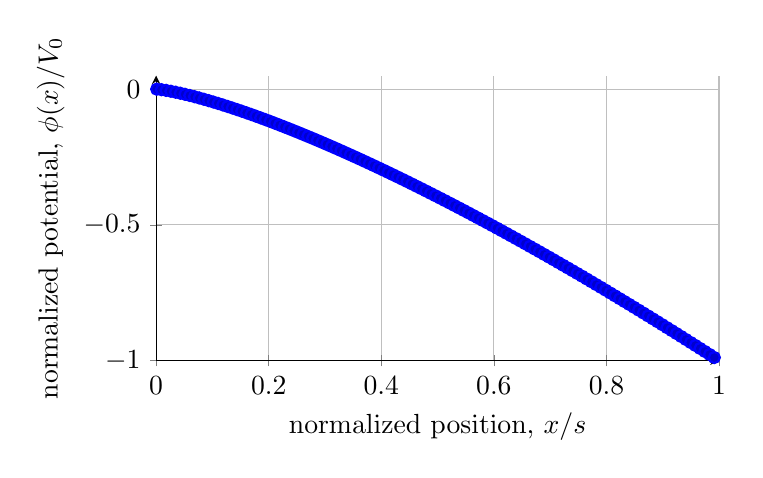
\begin{tikzpicture}
\begin{axis}[
 width=0.72\linewidth,
 height=5.2cm,
 xlabel={normalized position, $x/s$},
 ylabel={normalized potential, $\phi(x)/V_{0}$},
 domain=0.001:1,
 samples=120,
 grid=both,
 axis lines=left,
 xmin=0, xmax=1,
 ymin=-1, ymax=0.05,
 every axis plot/.append style={black, thick},
]
\addplot {-(x)^(4/3)};
\end{axis}
\end{tikzpicture}
\caption{Normalized Child--Langmuir sheath potential profile $\phi(x)/V_{0} = -(x/s)^{4/3}$ from the analytic solution of Eq.~\eqref{eq:cl-ode}, plotted from the sheath edge ($x/s=0$) to the wall ($x/s=1$); a direct evaluation of the closed-form expression, not measured or simulated data.}
\label{fig:child-langmuir-profile}
\end{figure}

\subsection{Regions of the plasma-boundary transition}

Figure~\ref{fig:sheath-regions} summarizes the full spatial structure of the plasma-wall transition: a quasineutral bulk plasma sourcing ions essentially at rest; a quasineutral presheath, extending over a scale much larger than $\lambda_{\mathrm{D}}$, across which the weak ambipolar field accelerates ions to $u_{\mathrm{B}}$ while $\phi$ falls by $T_{\mathrm{e}}/2e$; and the non-neutral sheath, extending only a few to a few tens of $\lambda_{\mathrm{D}}$, across which essentially the entire remaining drop $V_{0}$ occurs \cite{ref0013,ref0023}.

\begin{figure}[htbp]
\centering
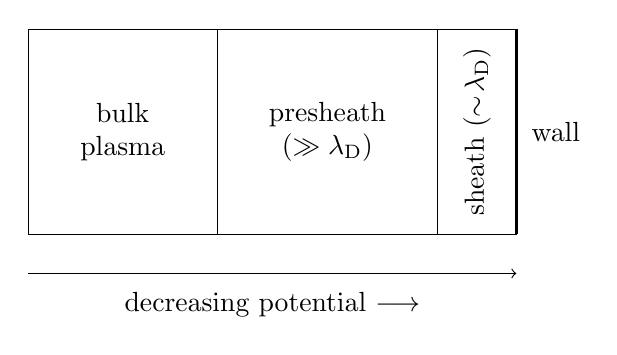
\begin{tikzpicture}[x=1cm, y=1cm]
\draw[black] (0,0) rectangle (2.4,2.6);
\draw[black] (2.4,0) rectangle (5.2,2.6);
\draw[black] (5.2,0) rectangle (6.2,2.6);
\draw[black, very thick] (6.2,0) -- (6.2,2.6);
\node[align=center] at (1.2,1.3) {bulk\\plasma};
\node[align=center] at (3.8,1.3) {presheath\\($\gg \lambda_{\mathrm{D}}$)};
\node[align=center, rotate=90] at (5.7,1.3) {sheath ($\sim\!\lambda_{\mathrm{D}}$)};
\node at (6.7,1.3) {wall};
\draw[black,->] (0,-0.5) -- (6.2,-0.5) node[midway, below=2pt]{};
\node at (3.1,-0.9) {decreasing potential $\longrightarrow$};
\end{tikzpicture}
\caption{Schematic (not to scale) plasma--presheath--sheath--wall spatial decomposition. The presheath spans a scale much larger than $\lambda_{\mathrm{D}}$; the sheath spans only a few to a few tens of $\lambda_{\mathrm{D}}$.}
\label{fig:sheath-regions}
\end{figure}

\subsection{Comparative scaling summary}

Table~\ref{tab:sheath-scaling} collects the scaling laws derived above and the collisional/magnetized generalizations below.

\begin{table}[htbp]
\centering
\caption{Sheath thickness and current scaling laws in the principal regimes discussed in this chapter. $s$: sheath thickness; $\lambda_{\mathrm{Ds}}$: sheath-edge Debye length; $V_{0}$: sheath voltage; $\ell_{\mathrm{i}}$: ion-neutral mean free path.}
\label{tab:sheath-scaling}
\begin{tabular}{lll}
\toprule
Regime & Thickness scaling & Governing relation \\
\midrule
Matrix sheath & $s \propto \lambda_{\mathrm{Ds}} (V_{0}/T_{\mathrm{e}})^{1/2}$ & Eq.~\eqref{eq:matrix-sheath} \\
Child--Langmuir sheath & $s \propto \lambda_{\mathrm{Ds}} (V_{0}/T_{\mathrm{e}})^{3/4}$ & Eq.~\eqref{eq:cl-thickness} \\
Collisional (mobility-limited) sheath & $s \propto \lambda_{\mathrm{Ds}}^{4/5} \ell_{\mathrm{i}}^{1/5} (V_{0}/T_{\mathrm{e}})^{2/5}$ & Section~\ref{sec:collisional} \\
Bohm--Chodura magnetic presheath & width $\sim \rho_{\mathrm{i}}$ (ion Larmor radius) & Section~\ref{sec:chodura} \\
\bottomrule
\end{tabular}
\end{table}

\section{Collisional Sheaths and the Bohm--Chodura Criterion}
\label{sec:collisional}

\subsection{Ion-neutral collisions in the presheath}

The derivation of Section~\ref{ch03-sec:bohm} assumed ions are collisionless across the presheath and sheath. In many technologically relevant plasmas -- moderate-pressure capacitively or inductively coupled discharges -- the ion-neutral mean free path $\ell_{\mathrm{i}}$ can be comparable to, or smaller than, the presheath length. Collisions drag on the ion fluid, requiring a larger presheath field to reach the sheath-edge criterion, and broaden $f_{\mathrm{i}}(v)$ at the sheath edge, since ions undergo their last collision at varying distances from the wall \cite{ref0009,ref0024}.

\subsection{The generalized collisional Bohm criterion}

A convenient generalization retains the fluid momentum equation but adds a friction term proportional to the ion-neutral collision frequency $\nu_{\mathrm{i}n}$:
\begin{equation}
m_{\mathrm{i}} n_{\mathrm{i}} u_{\mathrm{i}} \frac{\mathrm{d}u_{\mathrm{i}}}{\mathrm{d}x} = -e n_{\mathrm{i}} \frac{\mathrm{d}\phi}{\mathrm{d}x} - m_{\mathrm{i}} n_{\mathrm{i}} \nu_{\mathrm{i}n} u_{\mathrm{i}}.
\label{eq:collisional-momentum}
\end{equation}
Repeating the linear-stability argument of Section~\ref{ch03-sec:bohm} with Eq.~\eqref{eq:collisional-momentum} shows the marginal sheath-edge speed is modified from the simple $u_{\mathrm{B}}$ of Eq.~\eqref{ch03-eq:bohm-criterion}; in the constant-mean-free-path limit it becomes a function of $\lambda_{\mathrm{Ds}}/\ell_{\mathrm{i}}$, approaching $u_{\mathrm{B}}$ as $\lambda_{\mathrm{Ds}}/\ell_{\mathrm{i}} \to 0$ and falling somewhat below $u_{\mathrm{B}}$ as collisionality increases, since collisions supply part of the ``stiffening'' inertia alone provided in the collisionless case \cite{ref0009,ref0024,ref0015}. Two-fluid treatments retaining finite $T_{\mathrm{i}}$ show a warm-ion presheath both reduces the required sheath-edge velocity and modifies the density factor away from the cold-ion value $\exp(-1/2)$ \cite{ref0023}.

\subsection{Mobility-limited (high-pressure) sheath thickness}

In the opposite, strongly collisional limit, where the ion mean free path is much smaller than the sheath thickness, ion transport is dominated by mobility rather than free acceleration: $u_{\mathrm{i}} = \mu_{\mathrm{i}} E$. Repeating the Child--Langmuir derivation with this relation, the sheath thickness scales approximately as
\begin{equation}
s_{\mathrm{mob}} \propto \lambda_{\mathrm{Ds}}^{4/5}\, \ell_{\mathrm{i}}^{1/5} \left( \frac{e V_{0}}{k_{\mathrm{B}} T_{\mathrm{e}}} \right)^{2/5},
\end{equation}
a weaker voltage dependence than the collisionless $3/4$-power law, reflecting additional damping by collisions with the neutral background \cite{ref0024}. The resulting reduction of net ion flux to the wall as collisionality increases has direct consequences for $\Gamma_{E}$, treated as a correction factor in later chapters \cite{ref0024}.

\subsection{Magnetized presheath and the Chodura layer}
\label{sec:chodura}

When a static magnetic field $\mathbf{B}$ is present at the plasma boundary -- fusion divertors, magnetized processing plasmas, Hall-effect thrusters -- the presheath acquires structure not captured by unmagnetized theory. If $\mathbf{B}$ is oblique to the wall (angle $\alpha \ne 90^{\circ}$), ion gyromotion introduces a new intermediate scale, the ion Larmor radius $\rho_{\mathrm{i}} = m_{\mathrm{i}} v_{\perp}/(eB)$, with $\lambda_{\mathrm{D}} \ll \rho_{\mathrm{i}} \ll$ (collisional presheath scale). Chodura showed a new, quasineutral \emph{magnetic presheath} of width $\sim \rho_{\mathrm{i}}$ must be inserted between the traditional presheath and the electrostatic Debye sheath, within which ions accelerate along the field line while deflected by $\mathbf{E}\times\mathbf{B}$ and gyro-motion toward the wall \cite{ref0017,ref0018}.

\subsection{The Bohm--Chodura criterion}

Within this magnetic presheath, the generalized Bohm--Chodura criterion requires the ion drift component \emph{along the magnetic field}, $u_{\parallel}$, to reach the acoustic speed at the entrance to the magnetic presheath,
\begin{equation}
u_{\parallel} \ge u_{\mathrm{B}} = \sqrt{\frac{k_{\mathrm{B}} T_{\mathrm{e}}}{m_{\mathrm{i}}}},
\label{eq:chodura-parallel}
\end{equation}
while quasineutrality and the magnetic presheath geometry simultaneously require the ion velocity component \emph{normal to the wall}, $u_{\perp,\mathrm{wall}}$, to reach at least $u_{\mathrm{B}} \sin\alpha$ by the time ions reach the Debye-scale electrostatic sheath edge \cite{ref0017,ref0018}:
\begin{equation}
u_{\perp,\mathrm{wall}} \ge u_{\mathrm{B}} \sin\alpha.
\label{eq:chodura-normal}
\end{equation}
As $\alpha \to 90^{\circ}$, Eqs.~\eqref{eq:chodura-parallel} and~\eqref{eq:chodura-normal} coincide and the unmagnetized Bohm criterion is recovered; for grazing incidence ($\alpha \to 0$), the normal-velocity requirement weakens, since gyro-orbits carry ions only slowly toward the wall even though their parallel speed is already sonic \cite{ref0017,ref0018}. The magnetic presheath thus adds a fourth region, intermediate in scale ($\rho_{\mathrm{i}}$), to the spatial hierarchy of a magnetized, weakly collisional boundary plasma.

\section{Radio-Frequency and Capacitive Sheaths}

\subsection{Why time dependence matters}

The sheath theory developed so far is strictly a DC construction. Many technologically important plasmas are sustained or biased with radio-frequency (RF) power, from tens of kHz to hundreds of MHz, and the sheath adjacent to an RF-driven electrode oscillates in thickness and instantaneous voltage with the applied waveform. Whether ions respond quasi-statically, average over the oscillation, or respond in some intermediate fashion depends on the ratio of the ion transit time, $\tau_{\mathrm{i}} \sim s/u_{\mathrm{B}}$, to the RF period $\tau_{\mathrm{rf}} = 2\pi/\omega$.

\subsection{Frequency regimes}

In the \emph{low-frequency} regime, $\omega \tau_{\mathrm{i}} \ll 1$, ions cross the sheath in a small fraction of an RF cycle and respond essentially instantaneously: the sheath can be modelled at each instant by the DC matrix or Child--Langmuir relations, tracking $V(t) = V_{0} + V_{\mathrm{rf}} \sin(\omega t)$ \cite{ref0043}. In the opposite, \emph{high-frequency} regime, $\omega \tau_{\mathrm{i}} \gg 1$, ions need many RF periods to cross the sheath and respond only to the time-averaged field, so the sheath behaves as a nonlinear capacitor whose ion flux is frozen at its time-averaged Bohm value \cite{ref0043}. Most capacitively coupled sources -- typically driven at $\SI{13.56}{\mega\hertz}$ or higher -- operate near the high-frequency regime for heavy ions and the low-frequency or intermediate regime for light ions, so a single discharge can display different sheath dynamics for different ion masses simultaneously \cite{ref0038,ref0040}.

\subsection{The intermediate regime and sheath harmonics}

Neither limit is exact for $\omega \tau_{\mathrm{i}} \sim 1$, the \emph{intermediate} regime relevant to many practical frequencies and pressures. Kinetic and particle-in-cell simulations show the sheath develops significant harmonic content beyond the fundamental drive frequency, tied to the nonlinear, voltage-dependent impedance of the space-charge layer \cite{ref0040,ref0043}, underlying waveform-tailoring techniques that decouple control of ion flux from mean ion energy. Equivalent-circuit descriptions, representing the sheath as a voltage-dependent capacitor in series with a bulk plasma resistance and inductance, offer a compact framework for interpreting these dynamics without full kinetic simulation.

\subsection{Collisional and magnetized RF sheaths}

The collisional and magnetized generalizations of Section~\ref{sec:collisional} carry over, with added complexity, to the RF case. Collisional RF sheath models track the instantaneous balance between ion inertia, collisional drag, and the time-varying field, showing that increasing pressure both damps the sheath-oscillation amplitude and broadens the ion energy spread at the wall \cite{ref0043}. In magnetized RF discharges, interaction of the oscillating sheath field with ion and electron gyromotion introduces frequency-dependent modification of the Bohm--Chodura condition, while secondary electron emission from an RF-biased surface can substantially modify or disrupt the classical RF sheath structure at high emission yield, particularly for dielectric walls \cite{ref0038}.

\subsection{Self-bias, asymmetry, and battery effects}

An RF-driven electrode capacitively coupled to the plasma (unable to pass net DC current) must develop, in steady state, a DC self-bias such that time-averaged ion and electron currents balance -- analogous to the DC floating condition of Eq.~\eqref{eq:floating-potential} but for cycle-averaged fluxes. When the areas, capacitances, or waveforms of the two electrodes bounding an RF discharge are unequal -- the \emph{asymmetric} discharge -- the two sheaths do not carry equal time-averaged voltage, and a substantial DC self-bias develops across the smaller electrode, a sheath ``battery effect'' that adds directly to the sheath voltage seen by ions there, a handle for controlling mean ion bombardment energy independently of discharge power.

\subsection{Bimodal ion energy distributions}

The single most important consequence of RF sheath dynamics for this monograph is the modification it produces in the ion energy distribution function (IEDF) delivered to the wall, relative to the mono-energetic result of Eq.~\eqref{eq:ion-impact-energy}. In the low-frequency limit, ions respond to the full instantaneous voltage swing, and because they spend a disproportionate fraction of the cycle near the two turning points of $V(t)$ (where $\mathrm{d}V/\mathrm{d}t \to 0$), the IEDF develops two pronounced peaks -- a \emph{bimodal} distribution -- near $e(V_{0} - V_{\mathrm{rf}})$ and $e(V_{0}+V_{\mathrm{rf}})$ \cite{ref0055}. As driving frequency increases toward the high-frequency limit, ions can no longer follow the instantaneous field, the peaks narrow and merge, and the IEDF collapses toward a single peak centred on the time-averaged sheath voltage \cite{ref0055,ref0040}. This transition shows why a purely time-averaged treatment cannot predict the true ion energy flux delivered by an RF-driven boundary: the flux-weighted mean energy and second moment of $f_{\mathrm{i}}(v)$ depend on the entire waveform of $V(t)$ relative to $\tau_{\mathrm{i}}$, not merely its mean.

\section{Kinetic Corrections and Finite-Debye-Length Effects}

\subsection{Limits of the cold-ion fluid picture}

The derivation of Section~\ref{ch03-sec:bohm} idealized the ion population as a cold, mono-energetic fluid entering the sheath at a single speed $u_{0}$. Real ion populations, even collisionless, arrive at the sheath edge with a spread of velocities set by their birth location in the presheath, since an ion born at $x'$ and accelerated freely to $x=0$ carries a speed set by the potential drop between $x'$ and $0$. The correct kinetic description replaces $u_{0}$ with a full velocity distribution $f_{\mathrm{i}}(v)$ at the sheath edge, normalized so $n_{\mathrm{s}} = \int_{0}^{\infty} f_{\mathrm{i}}(v)\, \mathrm{d}v$, and the fluid Bohm criterion must be re-derived as a moment condition \cite{ref0006}.

\subsection{The kinetic (Harrison--Thompson) Bohm criterion}

Repeating the linearized-Poisson argument with the ion density expressed as a velocity-space integral over $f_{\mathrm{i}}(v)$, the marginal-stability condition generalizes to an inequality on the $v^{-2}$-weighted moment:
\begin{equation}
\boxed{\, \int_{0}^{\infty} \frac{f_{\mathrm{i}}(v)}{v^{2}}\, \mathrm{d}v \;\le\; \frac{n_{\mathrm{s}}\, m_{\mathrm{i}}}{k_{\mathrm{B}} T_{\mathrm{e}}} \,}.
\label{eq:kinetic-bohm}
\end{equation}
Equation~\eqref{eq:kinetic-bohm} is the kinetic form of the Bohm criterion, sometimes attributed to Harrison and Thompson \cite{ref0001}. It reduces to the fluid criterion of Eq.~\eqref{ch03-eq:bohm-criterion} for a mono-energetic distribution $f_{\mathrm{i}}(v) = n_{\mathrm{s}}\, \delta(v-u_{0})$, for which the integral evaluates to $n_{\mathrm{s}}/u_{0}^{2}$. For a distribution with any spread, the $v^{-2}$ weighting means the criterion is dominated by the \emph{slowest} ions present: a small slow population can violate it even when the bulk, and the flux-averaged mean speed, comfortably exceeds $u_{\mathrm{B}}$ -- motivating fully kinetic treatments of the presheath--sheath transition via the Vlasov equation \cite{ref0659}.

\subsection{The Tonks--Langmuir kinetic model}

The paradigmatic fully kinetic treatment of the presheath--sheath system is the Tonks--Langmuir model, in which ions are created by ionization of a cold background at a spatially varying rate and fall freely, without collisions, from their birth point onward. Because an ion at $x$ may have been born anywhere between the plasma centre and $x$, the model self-consistently generates a broad, non-mono-energetic $f_{\mathrm{i}}(v;x)$ at every point, and whether the kinetic Bohm criterion, Eq.~\eqref{eq:kinetic-bohm}, is satisfied \emph{as a consequence of} the free-fall ionization kinematics -- rather than imposed separately -- has long been debated. Extensions to non-Maxwellian electron populations show the electron energy distribution shape feeds directly into the ionization source term and hence into the resulting ion distribution, altering numerical prefactors while leaving the qualitative structure intact.

\subsection{Continuum-kinetic and Vlasov simulation approaches}

Because the presheath-to-sheath transition spans several orders of magnitude in length scale and involves a genuinely non-Maxwellian, evolving ion distribution, it is a natural target for direct numerical solution of the Vlasov (collisionless kinetic) equation, alone or coupled to a Boltzmann collision operator for finite collisionality \cite{ref0670}. Continuum-kinetic (grid-based) discretizations of the Vlasov--Poisson system resolve the sheath and presheath self-consistently, requiring velocity-space resolution fine enough to avoid spurious noise near the sharp, nearly singular ion distribution at the sheath edge; bi-species Vlasov--Poisson--Boltzmann formulations extend this to explicitly collisional sheaths.

\subsection{Kinetic effects in magnetized and grazing-angle geometries}

The magnetic presheath problem of Section~\ref{sec:chodura} is intrinsically kinetic at grazing field angles, because ion gyro-orbits carrying particles toward the wall have a radius $\rho_{\mathrm{i}}$ comparable to the presheath scale itself, so a fluid (guiding-centre) description becomes progressively less accurate as $\alpha \to 0$. Large-gyro-orbit kinetic models, retaining the full cyclotron trajectory, show the ion distribution delivered to the Debye sheath at grazing incidence departs substantially from the shifted-Maxwellian or mono-energetic pictures used in the fluid Bohm--Chodura derivation, a departure confirmed qualitatively by laser-induced-fluorescence measurements of the presheath ion velocity distribution.

\subsection{Finite Debye-length (finite $\lambda_{\mathrm{D}}/L$) effects}

Every result derived in Sections~\ref{ch03-sec:bohm} through the present section relies on the formal scale separation $\lambda_{\mathrm{D}} \ll L$, where $L$ is the presheath or system length scale; the sharp division into a quasineutral presheath and a non-neutral sheath is an asymptotic statement valid as $\lambda_{\mathrm{D}}/L \to 0$. For finite, non-negligible $\lambda_{\mathrm{D}}/L$ -- relevant to small discharges, low-density plasmas, or dust-grain and probe sheaths only modestly larger than $\lambda_{\mathrm{D}}$ -- quasineutrality is not exactly satisfied anywhere, presheath and sheath blend continuously without a sharp edge, and the Bohm criterion must be reformulated as an asymptotic matching statement rather than a boundary condition at a precise location \cite{ref0012}. Systematic treatments solving Eq.~\eqref{ch03-eq:poisson-full} show the practical threshold ion speed approaches $u_{\mathrm{B}}$ smoothly from above as $\lambda_{\mathrm{D}}/L \to 0$, with calculable finite-size corrections to the sheath-edge density and potential offset. Related considerations govern the electron-rich, or electron-sheath, regime near strongly electron-emitting or highly negatively charged boundaries, where the roles of light and heavy species reverse \cite{ref0006}.

\subsection{Practical implications for the fluid picture used elsewhere}

The kinetic and finite-Debye-length corrections surveyed here do not overturn the fluid framework of Sections~\ref{ch03-sec:bohm}--\ref{sec:collisional}; rather, they define its domain of validity. For the great majority of laboratory low-temperature plasmas relevant to ion energy flux measurement -- $\lambda_{\mathrm{D}}$ typically tens of micrometres to a few millimetres, system scales centimetres or more -- the fluid Bohm criterion and Child--Langmuir thickness scaling of Eq.~\eqref{eq:cl-thickness} remain quantitatively reliable and underlie the ion energy flux formalism developed in the following chapter. Kinetic corrections become essential in strongly grazing magnetic field angles, RF sheaths at low $\omega\tau_{\mathrm{i}}$ with broad IEDFs, multi-ion-species and electronegative plasmas, and any boundary not overwhelmingly larger than $\lambda_{\mathrm{D}}$.

\subsection{Consequences for the energy-flux moment}

Returning to Eq.~\eqref{eq:energy-flux-moments}, each correction surveyed here reshapes the second (energy-weighted) moment $\Gamma_{E}$ relative to the idealized delta-function prediction of Eq.~\eqref{eq:ion-impact-energy}. Ion-neutral collisions (Section~\ref{sec:collisional}) remove high-energy ions from the beam via charge exchange and momentum-transfer scattering while injecting slow, newly created ions, broadening $f_{\mathrm{i}}(v)$ at the wall toward lower energies and lowering $\Gamma_{E}$ relative to $\Gamma_{\mathrm{i}} E_{\mathrm{i}}$ \cite{ref0024}. The Bohm--Chodura magnetized criterion (Section~\ref{sec:chodura}) instead redistributes energy between wall-normal and wall-tangential velocity components: since only the normal component contributes to the flux crossing the Debye sheath while the full speed contributes to kinetic energy, oblique magnetic incidence generally reduces the normal-direction energy flux at fixed sheath voltage, more pronounced near grazing incidence \cite{ref0017,ref0018}. The RF sheaths of Section~6 modify $\Gamma_{E}$ differently again: the correct energy flux is a flux-weighted average over the periodic waveform, $\Gamma_{E} \propto \langle V(t)^{3/2} \rangle_{t}$ in the space-charge-limited regime, systematically larger than $\langle V(t) \rangle_{t}^{3/2}$ by the convexity of $V^{3/2}$ (Jensen's inequality) \cite{ref0055}. Finally, the kinetic corrections act principally on the low-velocity tail of $f_{\mathrm{i}}(v)$ and so have a comparatively modest direct effect on $\Gamma_{E}$ (dominated by the high-velocity tail), even though that same low-velocity tail controls the marginal Bohm criterion -- why sheath-edge diagnostics testing the Bohm criterion and wall-plane diagnostics quantifying $\Gamma_{E}$ probe weakly correlated features of the same distribution.

\section{Summary}

This chapter developed the theory of the plasma sheath from the elementary flux-balance argument for its existence through to its full kinetic and magnetized generalizations. The disparity between electron and ion thermal mobilities forces the formation of a non-neutral boundary layer that establishes current balance at any material surface; the resulting floating, wall, and plasma potentials are fixed by the exponential retardation of the electron flux against the comparatively rigid ion flux delivered by the Bohm criterion, $u_{0} \ge u_{\mathrm{B}} = \sqrt{k_{\mathrm{B}} T_{\mathrm{e}}/m_{\mathrm{i}}}$, derived from requiring the space-charge Poisson equation admit a monotonic solution. Its enforcement by a quasineutral presheath -- imposing a universal potential drop of $T_{\mathrm{e}}/2$ and a sheath-edge density reduction of $\exp(-1/2)$ in the cold-ion, collisionless limit -- accelerates thermal ions to the sheath entrance condition, and the sheath itself has a thickness of order a few Debye lengths in the matrix approximation, growing as $(V_{0}/T_{\mathrm{e}})^{3/4}$ in the self-consistent Child--Langmuir regime.

Collisions relax and reshape this picture toward a mobility-limited sheath at high pressure, while an oblique magnetic field imposes an entirely new intermediate structure, the Chodura magnetic presheath, governed by the joint Bohm--Chodura conditions on parallel and wall-normal ion velocity. Time-dependent RF excitation interpolates between a quasi-static, DC-like sheath at low frequency and a time-averaged, capacitor-like sheath at high frequency, with the intermediate regime responsible for the characteristic bimodal ion energy distributions at capacitively coupled discharge walls. Kinetic corrections -- most importantly the Harrison--Thompson generalization of the Bohm criterion to a $v^{-2}$-weighted moment of $f_{\mathrm{i}}(v)$ -- refine, and in several regimes (grazing magnetic incidence, low-frequency RF, finite $\lambda_{\mathrm{D}}/L$, multi-species and electronegative plasmas) qualitatively supersede, the cold-fluid picture.

In every regime treated here, the sheath converts a thermal, near-isotropic ion population in the plasma bulk into a directed, accelerated flux striking the wall with an energy set by the local sheath voltage (and, more generally, by the full time- and velocity-resolved history of that voltage as sampled by $f_{\mathrm{i}}(v)$). It is this conversion -- quantified through the particle flux $\Gamma_{\mathrm{i}} = n_{\mathrm{s}} u_{\mathrm{B}}$ and the mean ion impact energy of Eq.~\eqref{eq:ion-impact-energy}, or their collisional, magnetized, and RF-modulated generalizations -- that defines $\Gamma_{E}$ at the heart of this monograph, and forms the theoretical foundation for the sensor design and diagnostics developed in the chapters that follow.
